\documentclass[tikz,border=6pt]{standalone}
\usepackage[T1]{fontenc}
\usepackage{lmodern}
\usepackage{amsmath,amssymb}
\usetikzlibrary{arrows.meta,angles,quotes,calc,positioning}
\definecolor{axis}{HTML}{40515F}
\definecolor{grid}{HTML}{DDE4E8}
\definecolor{blue}{HTML}{3568D4}
\definecolor{coral}{HTML}{EF626C}
\definecolor{teal}{HTML}{2A9D8F}
\definecolor{gold}{HTML}{D89432}
\definecolor{purple}{HTML}{7357C8}
\tikzset{
  axisline/.style={axis, line width=.85pt, -{Stealth[length=3mm]}},
  guide/.style={axis!45, line width=.75pt, dashed},
  vector/.style={line width=1.5pt, -{Stealth[length=3mm]}},
  dot/.style={circle, fill=white, draw, line width=1.15pt, inner sep=2.15pt},
  label/.style={font=\large},
  smalllabel/.style={font=\normalsize}
}
\begin{document}

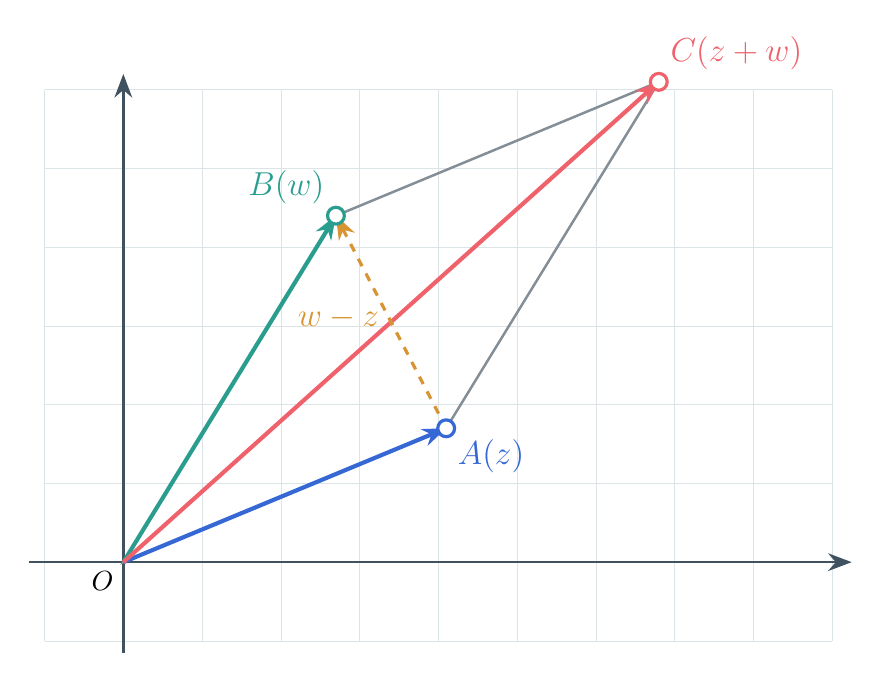
\begin{tikzpicture}[x=1cm,y=1cm]
  \draw[step=1cm,grid,very thin] (-1,-1) grid (9,6);
  \draw[axisline] (-1.2,0)--(9.25,0);
  \draw[axisline] (0,-1.15)--(0,6.2);
  \coordinate (O) at (0,0);
  \coordinate (A) at (4.1,1.7);
  \coordinate (B) at (2.7,4.4);
  \coordinate (C) at ($(A)+(B)$);
  \draw[axis!65,line width=.9pt] (O)--(A)--(C)--(B)--cycle;
  \draw[vector,blue] (O)--(A);
  \draw[vector,teal] (O)--(B);
  \draw[vector,coral] (O)--(C);
  \draw[gold,line width=1.15pt,dashed,-{Stealth[length=3mm]}] (A)--(B);
  \node[dot,draw=blue] at (A) {};
  \node[dot,draw=teal] at (B) {};
  \node[dot,draw=coral] at (C) {};
  \node[label,blue,below right=1pt of A] {$A(z)$};
  \node[label,teal,above left=1pt of B] {$B(w)$};
  \node[label,coral,above right=1pt of C] {$C(z+w)$};
  \node[label,gold,left] at ($(A)!.52!(B)$) {$w-z$};
  \node[smalllabel,below left] at (O) {$O$};
\end{tikzpicture}
\end{document}
